\section{keyboard Class Reference}
\label{classkeyboard}\index{keyboard@{keyboard}}
{\tt \#include $<$keyboard.h$>$}

Inheritance diagram for keyboard:\begin{figure}[H]
\begin{center}
\leavevmode
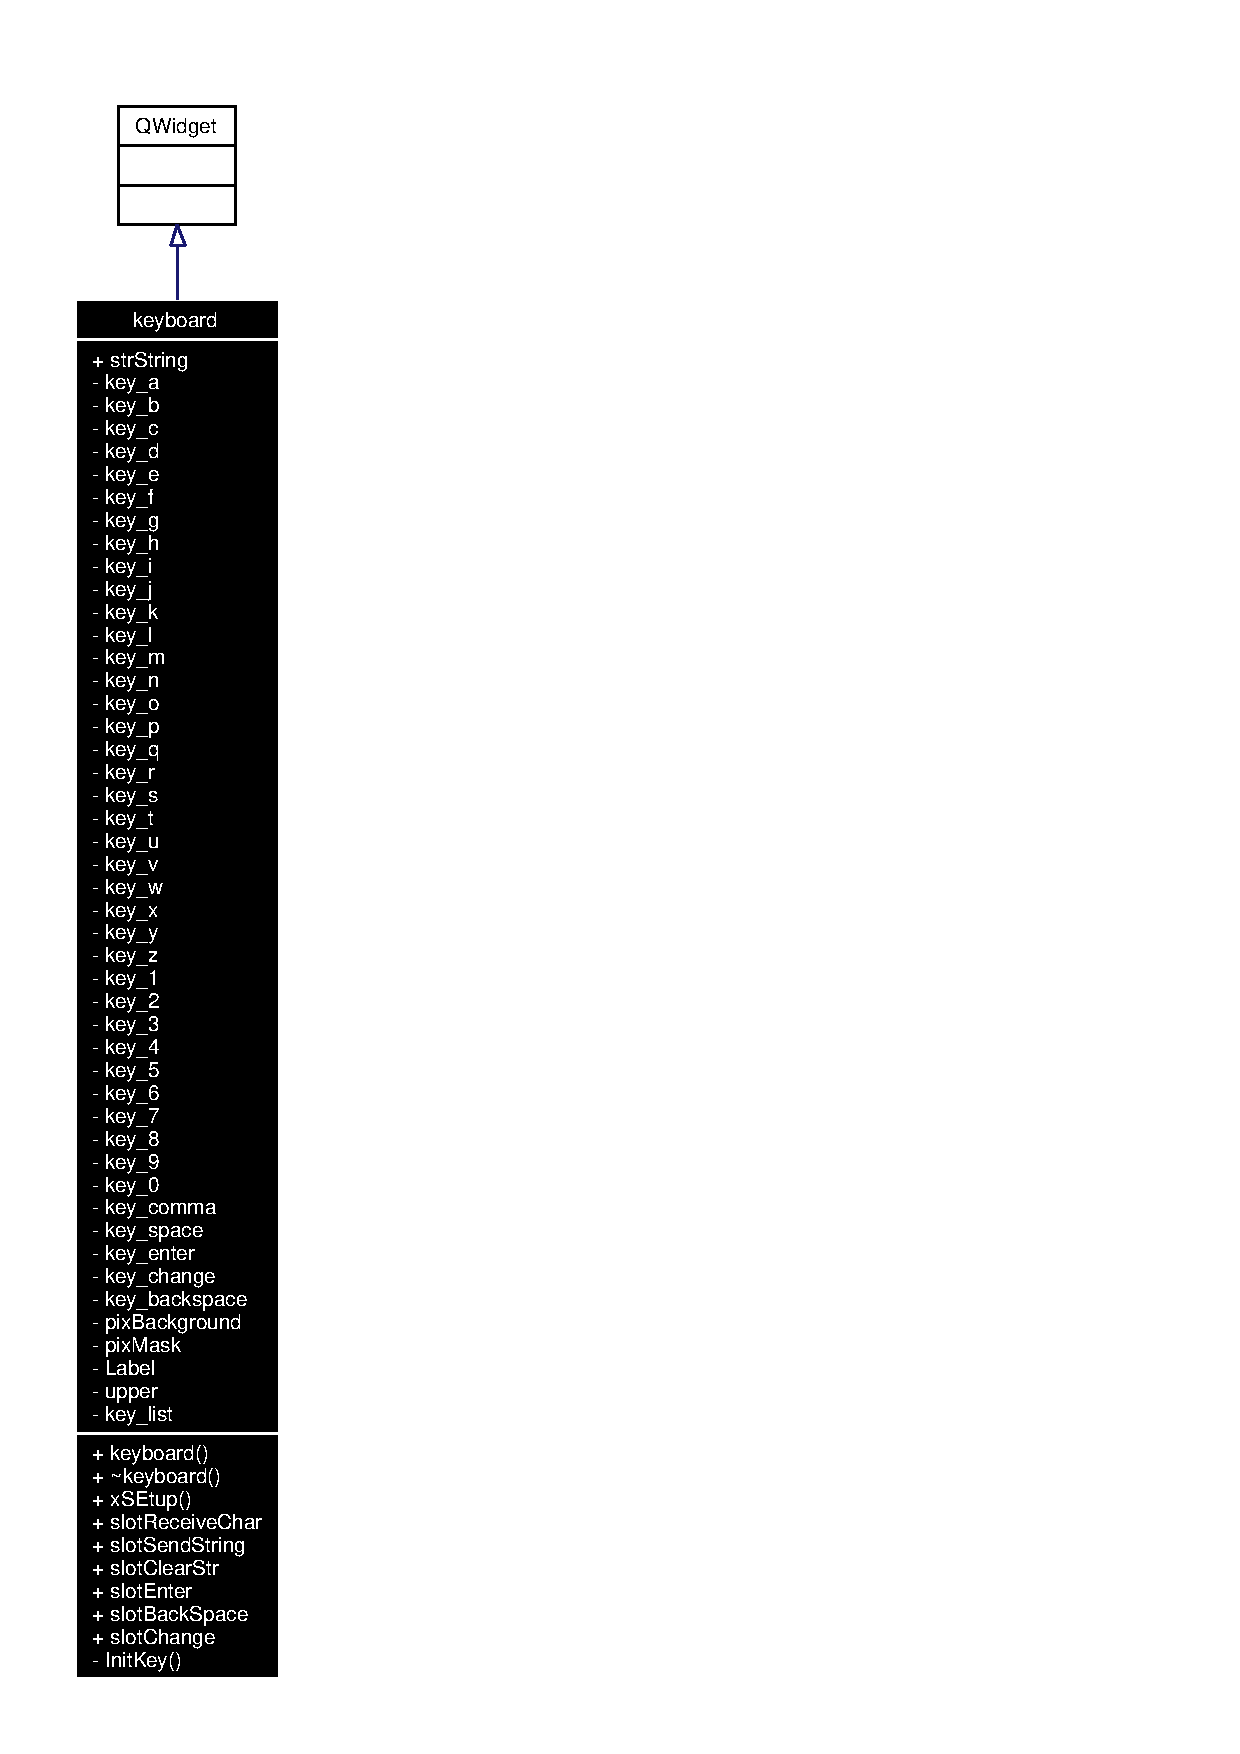
\includegraphics[width=67pt]{classkeyboard__inherit__graph}
\end{center}
\end{figure}
Collaboration diagram for keyboard:\begin{figure}[H]
\begin{center}
\leavevmode
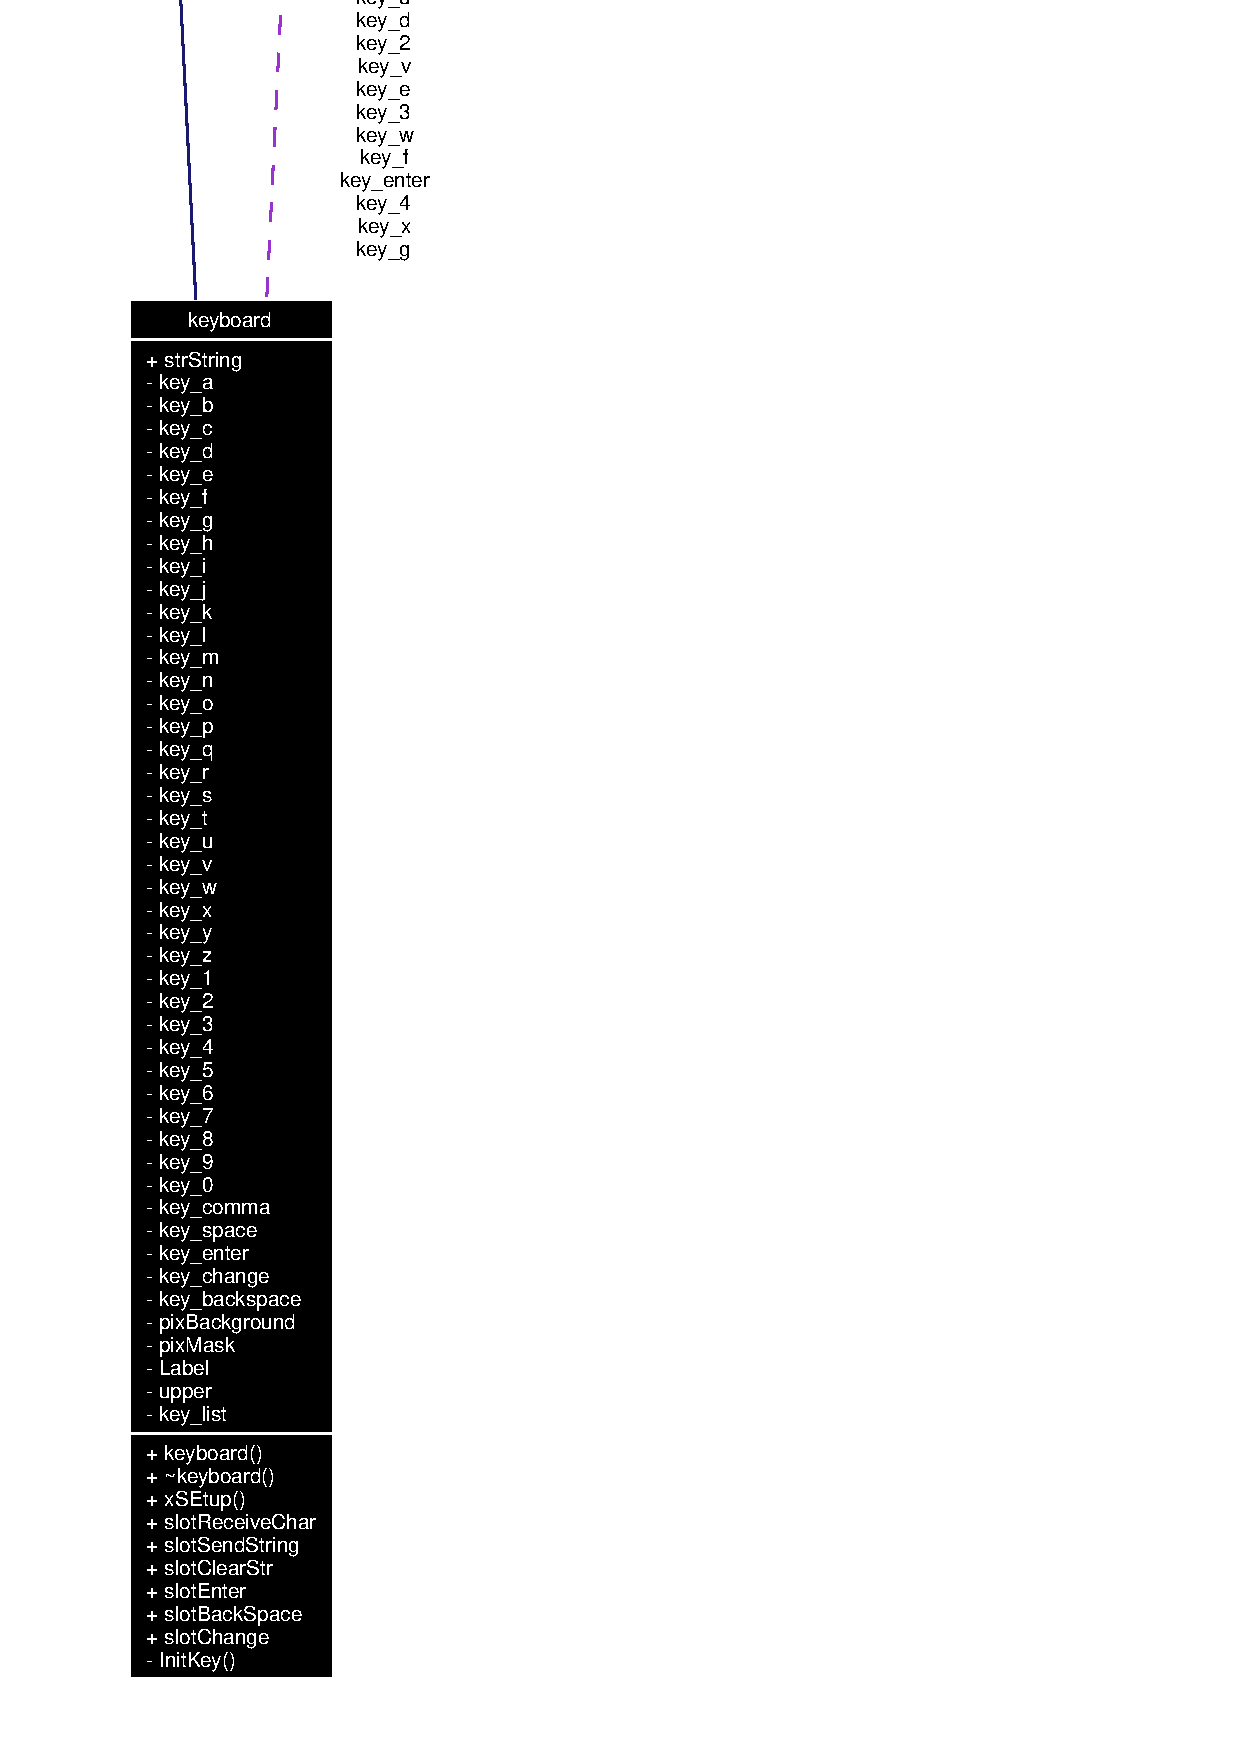
\includegraphics[width=114pt]{classkeyboard__coll__graph}
\end{center}
\end{figure}


\subsection{Detailed Description}
\begin{Desc}
\item[Author:]root \end{Desc}




Definition at line 36 of file keyboard.h.\subsection*{Public Slots}
\begin{CompactItemize}
\item 
void {\bf slot\-Receive\-Char} (QString str\_\-char)
\item 
void {\bf slot\-Send\-String} ()
\item 
void {\bf slot\-Clear\-Str} ()
\item 
void {\bf slot\-Enter} ()
\item 
void {\bf slot\-Back\-Space} ()
\item 
void {\bf slot\-Change} ()
\end{CompactItemize}
\subsection*{Signals}
\begin{CompactItemize}
\item 
void {\bf signal\-String} (QString)
\item 
void {\bf signal\-Enter} ()
\end{CompactItemize}
\subsection*{Public Member Functions}
\begin{CompactItemize}
\item 
{\bf keyboard} ({\bf QWidget} $\ast$parent=0, const char $\ast$name=0)
\item 
{\bf $\sim$keyboard} ()
\item 
void {\bf x\-SEtup} ()
\end{CompactItemize}
\subsection*{Public Attributes}
\begin{CompactItemize}
\item 
QString {\bf str\-String}
\end{CompactItemize}
\subsection*{Private Member Functions}
\begin{CompactItemize}
\item 
void {\bf Init\-Key} ()
\end{CompactItemize}
\subsection*{Private Attributes}
\begin{CompactItemize}
\item 
{\bf keyboard\_\-key} $\ast$ {\bf key\_\-a}
\item 
{\bf keyboard\_\-key} $\ast$ {\bf key\_\-b}
\item 
{\bf keyboard\_\-key} $\ast$ {\bf key\_\-c}
\item 
{\bf keyboard\_\-key} $\ast$ {\bf key\_\-d}
\item 
{\bf keyboard\_\-key} $\ast$ {\bf key\_\-e}
\item 
{\bf keyboard\_\-key} $\ast$ {\bf key\_\-f}
\item 
{\bf keyboard\_\-key} $\ast$ {\bf key\_\-g}
\item 
{\bf keyboard\_\-key} $\ast$ {\bf key\_\-h}
\item 
{\bf keyboard\_\-key} $\ast$ {\bf key\_\-i}
\item 
{\bf keyboard\_\-key} $\ast$ {\bf key\_\-j}
\item 
{\bf keyboard\_\-key} $\ast$ {\bf key\_\-k}
\item 
{\bf keyboard\_\-key} $\ast$ {\bf key\_\-l}
\item 
{\bf keyboard\_\-key} $\ast$ {\bf key\_\-m}
\item 
{\bf keyboard\_\-key} $\ast$ {\bf key\_\-n}
\item 
{\bf keyboard\_\-key} $\ast$ {\bf key\_\-o}
\item 
{\bf keyboard\_\-key} $\ast$ {\bf key\_\-p}
\item 
{\bf keyboard\_\-key} $\ast$ {\bf key\_\-q}
\item 
{\bf keyboard\_\-key} $\ast$ {\bf key\_\-r}
\item 
{\bf keyboard\_\-key} $\ast$ {\bf key\_\-s}
\item 
{\bf keyboard\_\-key} $\ast$ {\bf key\_\-t}
\item 
{\bf keyboard\_\-key} $\ast$ {\bf key\_\-u}
\item 
{\bf keyboard\_\-key} $\ast$ {\bf key\_\-v}
\item 
{\bf keyboard\_\-key} $\ast$ {\bf key\_\-w}
\item 
{\bf keyboard\_\-key} $\ast$ {\bf key\_\-x}
\item 
{\bf keyboard\_\-key} $\ast$ {\bf key\_\-y}
\item 
{\bf keyboard\_\-key} $\ast$ {\bf key\_\-z}
\item 
{\bf keyboard\_\-key} $\ast$ {\bf key\_\-1}
\item 
{\bf keyboard\_\-key} $\ast$ {\bf key\_\-2}
\item 
{\bf keyboard\_\-key} $\ast$ {\bf key\_\-3}
\item 
{\bf keyboard\_\-key} $\ast$ {\bf key\_\-4}
\item 
{\bf keyboard\_\-key} $\ast$ {\bf key\_\-5}
\item 
{\bf keyboard\_\-key} $\ast$ {\bf key\_\-6}
\item 
{\bf keyboard\_\-key} $\ast$ {\bf key\_\-7}
\item 
{\bf keyboard\_\-key} $\ast$ {\bf key\_\-8}
\item 
{\bf keyboard\_\-key} $\ast$ {\bf key\_\-9}
\item 
{\bf keyboard\_\-key} $\ast$ {\bf key\_\-0}
\item 
{\bf keyboard\_\-key} $\ast$ {\bf key\_\-comma}
\item 
{\bf keyboard\_\-key} $\ast$ {\bf key\_\-space}
\item 
{\bf keyboard\_\-key} $\ast$ {\bf key\_\-enter}
\item 
{\bf keyboard\_\-key} $\ast$ {\bf key\_\-change}
\item 
{\bf keyboard\_\-key} $\ast$ {\bf key\_\-backspace}
\item 
QPixmap {\bf pix\-Background}
\item 
QBitmap {\bf pix\-Mask}
\item 
QLabel $\ast$ {\bf Label}
\item 
bool {\bf upper}
\item 
QPtr\-List$<$ {\bf keyboard\_\-key} $>$ {\bf key\_\-list}
\end{CompactItemize}


\subsection{Constructor \& Destructor Documentation}
\index{keyboard@{keyboard}!keyboard@{keyboard}}
\index{keyboard@{keyboard}!keyboard@{keyboard}}
\subsubsection{\setlength{\rightskip}{0pt plus 5cm}keyboard::keyboard ({\bf QWidget} $\ast$ {\em parent} = 0, const char $\ast$ {\em name} = 0)}\label{classkeyboard_keyboarda0}




Definition at line 67 of file keyboard.cpp.

References x\-SEtup().



\footnotesize\begin{verbatim}68  : QWidget(parent, name),strString(0)
69 {
70  xSEtup();
71 }
\end{verbatim}\normalsize 


Here is the call graph for this function:\begin{figure}[H]
\begin{center}
\leavevmode
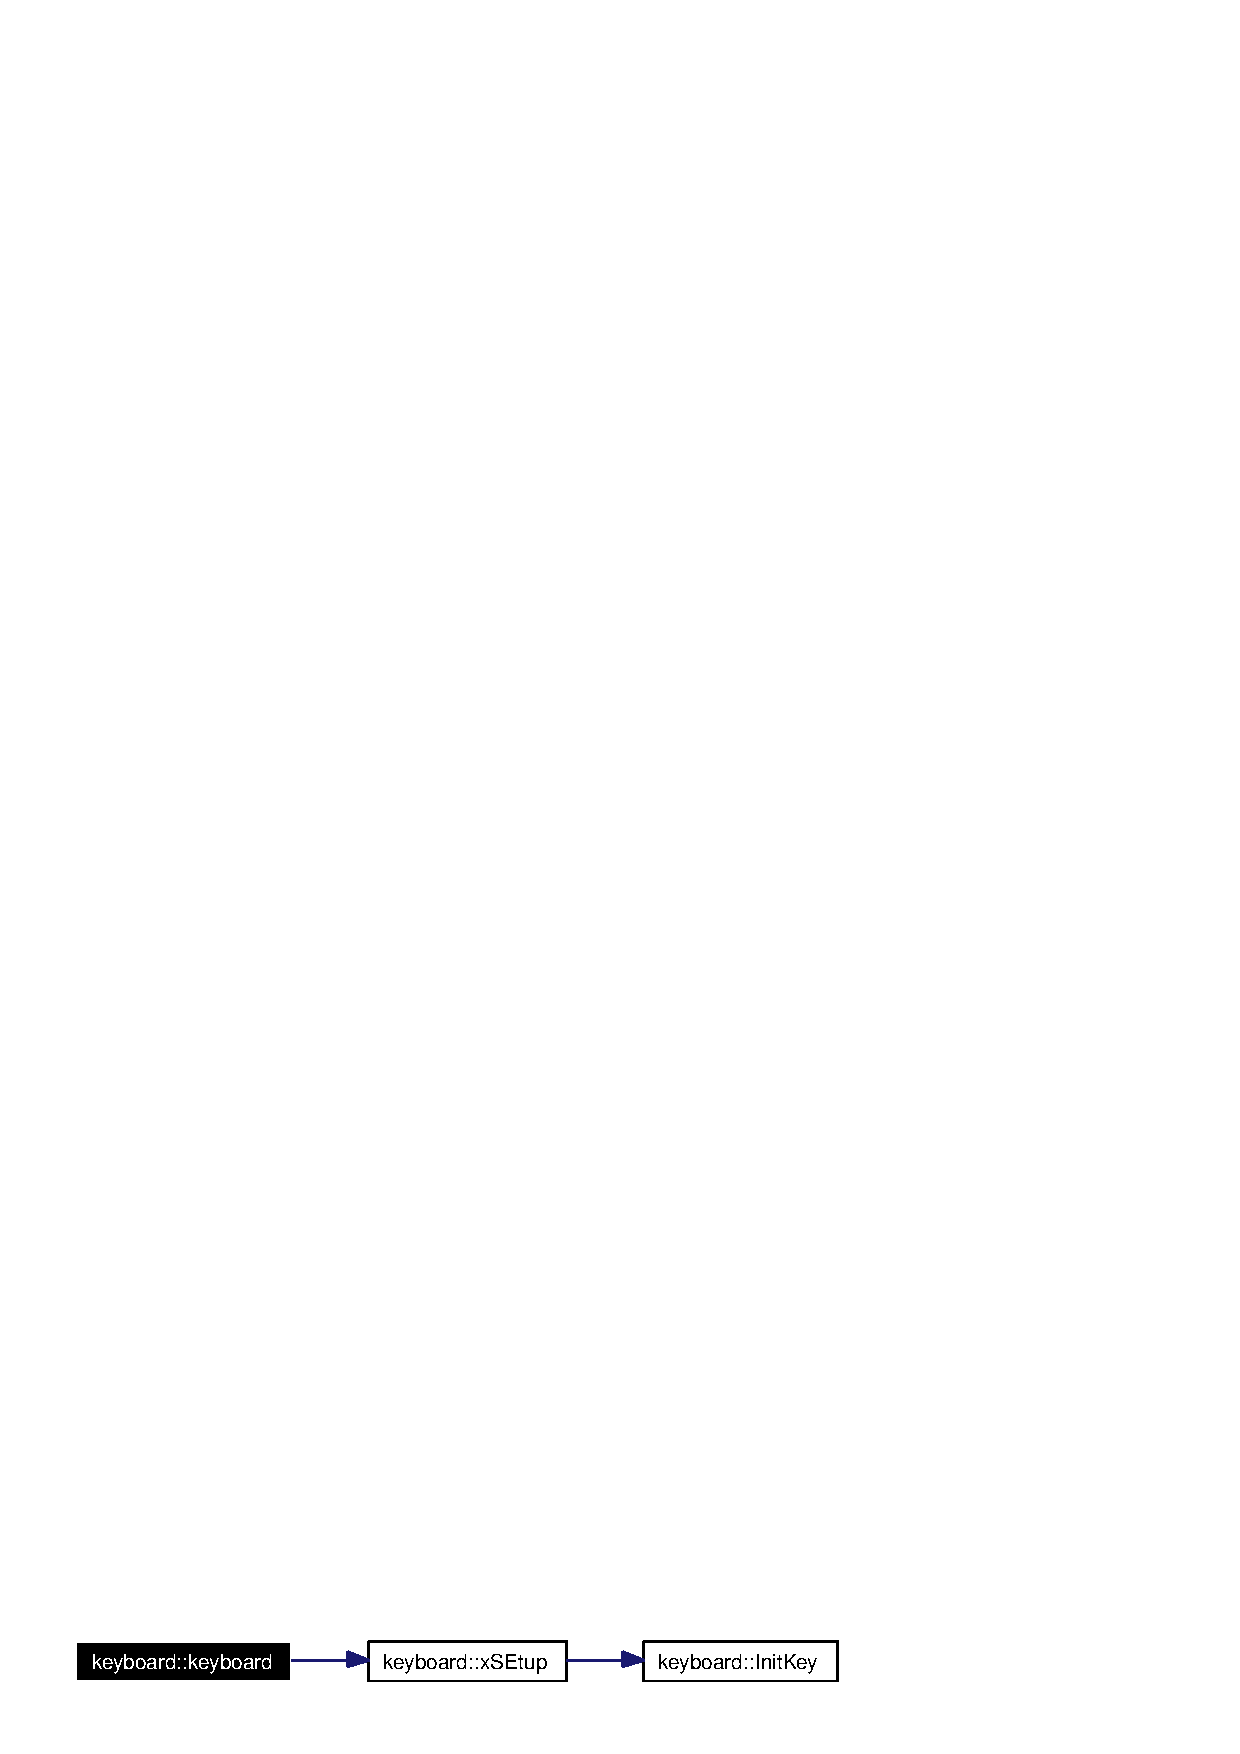
\includegraphics[width=201pt]{classkeyboard_keyboarda0_cgraph}
\end{center}
\end{figure}
\index{keyboard@{keyboard}!~keyboard@{$\sim$keyboard}}
\index{~keyboard@{$\sim$keyboard}!keyboard@{keyboard}}
\subsubsection{\setlength{\rightskip}{0pt plus 5cm}keyboard::$\sim${\bf keyboard} ()}\label{classkeyboard_keyboarda1}




Definition at line 74 of file keyboard.cpp.



\footnotesize\begin{verbatim}75 {
76 }
\end{verbatim}\normalsize 


\subsection{Member Function Documentation}
\index{keyboard@{keyboard}!InitKey@{InitKey}}
\index{InitKey@{InitKey}!keyboard@{keyboard}}
\subsubsection{\setlength{\rightskip}{0pt plus 5cm}void keyboard::Init\-Key ()\hspace{0.3cm}{\tt  [private]}}\label{classkeyboard_keyboardd0}




Definition at line 103 of file keyboard.cpp.

References key\_\-0, key\_\-1, key\_\-2, key\_\-3, key\_\-4, key\_\-5, key\_\-6, key\_\-7, key\_\-8, key\_\-9, key\_\-a, key\_\-b, key\_\-backspace, key\_\-c, key\_\-change, key\_\-comma, key\_\-d, key\_\-e, key\_\-enter, key\_\-f, key\_\-g, key\_\-h, key\_\-i, key\_\-j, key\_\-k, key\_\-l, key\_\-list, key\_\-m, key\_\-n, key\_\-o, key\_\-p, key\_\-q, key\_\-r, key\_\-s, key\_\-space, key\_\-t, key\_\-u, key\_\-v, key\_\-w, key\_\-x, key\_\-y, key\_\-z, Key\-Pos, Label, signal\-Enter(), slot\-Back\-Space(), slot\-Change(), slot\-Enter(), slot\-Receive\-Char(), and keyboard\_\-key::slot\-Set\-Pixmap().

Referenced by x\-SEtup().



\footnotesize\begin{verbatim}104 {
105    int keypos=0;
106    int width=58;
107    
108    //1->0
109    key_1=new keyboard_key(this,"A_a","1","!");
110    key_1->move(KeyPos[0][0]+width*keypos,KeyPos[0][1]);
111    key_1->show();
112    key_list.append(key_1);
113    connect(key_1,SIGNAL(signalSendChar(QString )),this,SLOT(slotReceiveChar(QString )));
114    keypos++;
115    
116    key_2=new keyboard_key(this,"A_a","2","@");
   key_2->move(KeyPos[0][0]+width*keypos,KeyPos[0][1]);
   key_2->show();
   key_list.append(key_2);
   connect(key_2,SIGNAL(signalSendChar(QString )),this,SLOT(slotReceiveChar(QString )));
   keypos++;
   
   key_3=new keyboard_key(this,"A_a","3","#");
117    key_3->move(KeyPos[0][0]+width*keypos,KeyPos[0][1]);
118    connect(key_3,SIGNAL(signalSendChar(QString )),this,SLOT(slotReceiveChar(QString )));
119    key_3->show();
120    key_list.append(key_3);
121    keypos++;
122    
123    key_4=new keyboard_key(this,"A_a","4","$");
124    key_4->move(KeyPos[0][0]+width*keypos,KeyPos[0][1]);
125    connect(key_4,SIGNAL(signalSendChar(QString )),this,SLOT(slotReceiveChar(QString )));
126    key_4->show();
127    key_list.append(key_4);
128    keypos++;
129    
130    key_5=new keyboard_key(this,"A_a","5","%");
131    key_5->move(KeyPos[0][0]+width*keypos,KeyPos[0][1]);
132    key_5->show();
133    key_list.append(key_5);
134    connect(key_5,SIGNAL(signalSendChar(QString )),this,SLOT(slotReceiveChar(QString )));
135    keypos++;
136    
137    key_6=new keyboard_key(this,"A_a","6","^");
138    key_6->move(KeyPos[0][0]+width*keypos,KeyPos[0][1]);
139    connect(key_6,SIGNAL(signalSendChar(QString )),this,SLOT(slotReceiveChar(QString )));
140    key_6->show();
141    key_list.append(key_6);
142    keypos++;
143    
144    key_7=new keyboard_key(this,"A_a","7","&");
145    key_7->move(KeyPos[0][0]+width*keypos,KeyPos[0][1]);
146    connect(key_7,SIGNAL(signalSendChar(QString )),this,SLOT(slotReceiveChar(QString )));
147    key_7->show();
148    key_list.append(key_7);
149    keypos++;
150    
151    key_8=new keyboard_key(this,"A_a","8","*");
152    key_8->move(KeyPos[0][0]+width*keypos,KeyPos[0][1]);
153    connect(key_8,SIGNAL(signalSendChar(QString )),this,SLOT(slotReceiveChar(QString )));
154    key_8->show();
155    key_list.append(key_8);
156    keypos++;
157    
158    key_9=new keyboard_key(this,"A_a","9","(");
159    key_9->move(KeyPos[0][0]+width*keypos,KeyPos[0][1]);
160    connect(key_9,SIGNAL(signalSendChar(QString )),this,SLOT(slotReceiveChar(QString )));
161    key_9->show();
162    key_list.append(key_9);
163    keypos++;
164    
165    key_0=new keyboard_key(this,"A_a","0",")");
166    key_0->move(KeyPos[0][0]+width*keypos,KeyPos[0][1]);
167    connect(key_0,SIGNAL(signalSendChar(QString )),this,SLOT(slotReceiveChar(QString )));
168    key_0->show();
169    key_list.append(key_0);
170    keypos++;
171    
172    
174    //Q->P
175    
176    keypos=0;
177    
178    key_q=new keyboard_key(this,"A_a","Q","q");
179    key_q->move(KeyPos[10][0]+width*keypos,KeyPos[10][1]);
180    connect(key_q,SIGNAL(signalSendChar(QString )),this,SLOT(slotReceiveChar(QString )));
181    key_q->show();
182    key_list.append(key_q);
183    keypos++;
184    
185    key_w=new keyboard_key(this,"A_a","W","w");
186    key_w->move(KeyPos[10][0]+width*keypos,KeyPos[10][1]);
187    connect(key_w,SIGNAL(signalSendChar(QString )),this,SLOT(slotReceiveChar(QString )));
188    key_w->show();
189    key_list.append(key_w);
190    keypos++;
191    
192    key_e=new keyboard_key(this,"A_a","E","e");
193    key_e->move(KeyPos[10][0]+width*keypos,KeyPos[10][1]);
194    connect(key_e,SIGNAL(signalSendChar(QString )),this,SLOT(slotReceiveChar(QString )));
195    key_e->show();
196    key_list.append(key_e);
197    keypos++;
198    
199    key_r=new keyboard_key(this,"A_a","R","r");
200    key_r->move(KeyPos[10][0]+width*keypos,KeyPos[10][1]);
201    connect(key_r,SIGNAL(signalSendChar(QString )),this,SLOT(slotReceiveChar(QString )));
202    key_r->show();
203    key_list.append(key_r);
204    keypos++;
205    
206    key_t=new keyboard_key(this,"A_a","T","t");
207    key_t->move(KeyPos[10][0]+width*keypos,KeyPos[10][1]);
208    connect(key_t,SIGNAL(signalSendChar(QString )),this,SLOT(slotReceiveChar(QString )));
209    key_t->show();
210    key_list.append(key_t);
211    keypos++;
212    
213    key_y=new keyboard_key(this,"A_a","Y","y");
214    key_y->move(KeyPos[10][0]+width*keypos,KeyPos[10][1]);
215    connect(key_y,SIGNAL(signalSendChar(QString )),this,SLOT(slotReceiveChar(QString )));
216    key_y->show();
217    key_list.append(key_y);
218    keypos++;
219    
220    key_u=new keyboard_key(this,"A_a","U","u");
221    key_u->move(KeyPos[10][0]+width*keypos,KeyPos[10][1]);
222    connect(key_u,SIGNAL(signalSendChar(QString )),this,SLOT(slotReceiveChar(QString )));
223    key_u->show();
224    key_list.append(key_u);
225    keypos++;
226    
227    key_i=new keyboard_key(this,"A_a","I","i");
228    key_i->move(KeyPos[10][0]+width*keypos,KeyPos[10][1]);
229    connect(key_i,SIGNAL(signalSendChar(QString )),this,SLOT(slotReceiveChar(QString )));
230    key_i->show();
231    key_list.append(key_i);
232    keypos++;
233    
234    key_o=new keyboard_key(this,"A_a","O","o");
235    key_o->move(KeyPos[10][0]+width*keypos,KeyPos[10][1]);
236    connect(key_o,SIGNAL(signalSendChar(QString )),this,SLOT(slotReceiveChar(QString )));
237    key_o->show();
238    key_list.append(key_o);
239    keypos++;
240    
241    key_p=new keyboard_key(this,"A_a","P","p");
242    key_p->move(KeyPos[10][0]+width*keypos,KeyPos[10][1]);
243    connect(key_p,SIGNAL(signalSendChar(QString )),this,SLOT(slotReceiveChar(QString )));
244    key_p->show();
245    key_list.append(key_p);
246    keypos++;
247    
249    //A->L
250    keypos=0;
251    
252    key_a=new keyboard_key(this,"A_a","A","a");
253    key_a->move(KeyPos[20][0]+width*keypos,KeyPos[20][1]);
254    connect(key_a,SIGNAL(signalSendChar(QString )),this,SLOT(slotReceiveChar(QString )));
255    key_a->show();
256    key_list.append(key_a);
257    keypos++;
258    
259    key_s=new keyboard_key(this,"A_a","S","s");
260    key_s->move(KeyPos[20][0]+width*keypos,KeyPos[20][1]);
261    connect(key_s,SIGNAL(signalSendChar(QString )),this,SLOT(slotReceiveChar(QString )));
262    key_s->show();
263    key_list.append(key_s);
264    keypos++;
265    
266    key_d=new keyboard_key(this,"A_a","D","d");
267    key_d->move(KeyPos[20][0]+width*keypos,KeyPos[20][1]);
268    connect(key_d,SIGNAL(signalSendChar(QString )),this,SLOT(slotReceiveChar(QString )));
269    key_d->show();
270    key_list.append(key_d);
271    keypos++;
272    
273    key_f=new keyboard_key(this,"A_a","F","f");
274    key_f->move(KeyPos[20][0]+width*keypos,KeyPos[20][1]);
275    connect(key_f,SIGNAL(signalSendChar(QString )),this,SLOT(slotReceiveChar(QString )));
276    key_f->show();
277    key_list.append(key_d);
278    keypos++;
279    
280    key_g=new keyboard_key(this,"A_a","G","g");
281    key_g->move(KeyPos[20][0]+width*keypos,KeyPos[20][1]);
282    connect(key_g,SIGNAL(signalSendChar(QString )),this,SLOT(slotReceiveChar(QString )));
283    key_g->show();
284    key_list.append(key_g);
285    keypos++;
286    
287    key_h=new keyboard_key(this,"A_a","H","h");
288    key_h->move(KeyPos[20][0]+width*keypos,KeyPos[20][1]);
289    connect(key_h,SIGNAL(signalSendChar(QString )),this,SLOT(slotReceiveChar(QString )));
290    key_h->show();
291    key_list.append(key_h);
292    keypos++;
293    
294    key_j=new keyboard_key(this,"A_a","J","j");
295    key_j->move(KeyPos[20][0]+width*keypos,KeyPos[20][1]);
296    connect(key_j,SIGNAL(signalSendChar(QString )),this,SLOT(slotReceiveChar(QString )));
297    key_j->show();
298    key_list.append(key_j);
299    keypos++;
300    
301    key_k=new keyboard_key(this,"A_a","K","k");
302    key_k->move(KeyPos[20][0]+width*keypos,KeyPos[20][1]);
303    connect(key_k,SIGNAL(signalSendChar(QString )),this,SLOT(slotReceiveChar(QString )));
304    key_k->show();
305    key_list.append(key_k);
306    keypos++;
307    
308    key_l=new keyboard_key(this,"A_a","L","l");
309    key_l->move(KeyPos[20][0]+width*keypos,KeyPos[20][1]);
310    connect(key_l,SIGNAL(signalSendChar(QString )),this,SLOT(slotReceiveChar(QString )));
311    key_l->show();
312    key_list.append(key_l);
313    keypos++;
314    
316    // Z->COMMA
317    keypos=0;
318    
319    key_z=new keyboard_key(this,"A_a","Z","z");
320    key_z->move(KeyPos[29][0]+width*keypos,KeyPos[29][1]);
321    connect(key_z,SIGNAL(signalSendChar(QString )),this,SLOT(slotReceiveChar(QString )));
322    key_z->show();
323    key_list.append(key_z);
324    keypos++;
325    
326    key_x=new keyboard_key(this,"A_a","X","x");
327    key_x->move(KeyPos[29][0]+width*keypos,KeyPos[29][1]);
328    connect(key_x,SIGNAL(signalSendChar(QString )),this,SLOT(slotReceiveChar(QString )));
329    key_x->show();
330    key_list.append(key_x);
331    keypos++;
332    
333    key_c=new keyboard_key(this,"A_a","C","c");
334    key_c->move(KeyPos[29][0]+width*keypos,KeyPos[29][1]);
335    connect(key_c,SIGNAL(signalSendChar(QString )),this,SLOT(slotReceiveChar(QString )));
336    key_c->show();
337    key_list.append(key_c);
338    keypos++;
339    
340    key_v=new keyboard_key(this,"A_a","V","v");
341    key_v->move(KeyPos[29][0]+width*keypos,KeyPos[29][1]);
342    connect(key_v,SIGNAL(signalSendChar(QString )),this,SLOT(slotReceiveChar(QString )));
343    key_v->show();
344    key_list.append(key_v);
345    keypos++;
346    
347    key_b=new keyboard_key(this,"A_a","B","b");
348    key_b->move(KeyPos[29][0]+width*keypos,KeyPos[29][1]);
349    connect(key_b,SIGNAL(signalSendChar(QString )),this,SLOT(slotReceiveChar(QString )));
350    key_b->show();
351    key_list.append(key_b);
352    keypos++;
353    
354    key_n=new keyboard_key(this,"A_a","N","n");
355    key_n->move(KeyPos[29][0]+width*keypos,KeyPos[29][1]);
356    connect(key_n,SIGNAL(signalSendChar(QString )),this,SLOT(slotReceiveChar(QString )));
357    key_n->show();
358    key_list.append(key_n);
359    keypos++;
360    
361    key_m=new keyboard_key(this,"A_a","M","m");
362    key_m->move(KeyPos[29][0]+width*keypos,KeyPos[29][1]);
363    connect(key_m,SIGNAL(signalSendChar(QString )),this,SLOT(slotReceiveChar(QString )));
364    key_m->show();
365    key_list.append(key_m);
366    keypos++;
367    
368    key_comma=new keyboard_key(this,"A_a",",",".");
369    key_comma->move(KeyPos[29][0]+width*keypos,KeyPos[29][1]);
370    connect(key_comma,SIGNAL(signalSendChar(QString )),this,SLOT(slotReceiveChar(QString )));
371    key_comma->show();
372    key_list.append(key_comma);
373    keypos++;
374    
375    
376    //SPACE 
377    QPixmap pixSpace=QPixmap("/root/kde_application/hdass08/skin/KeyBoardKey-Space.png");
378    QPixmap pixSpaceAcitve=QPixmap("/root/kde_application/hdass08/skin/KeyBoardKey-Space-Active.png");
379    key_space=new keyboard_key(this,"A_a"," "," ");
380    key_space->move(KeyPos[37][0],KeyPos[37][1]);
381    key_space->slotSetPixmap(pixSpace,pixSpaceAcitve);
382    connect(key_space,SIGNAL(signalSendChar(QString )),this,SLOT(slotReceiveChar(QString )));
383    key_space->show();
384    
385    //CHANGE
386    QPixmap pixChange=QPixmap("/root/kde_application/hdass08/skin/KeyBoardKey-Change.png");
387    QPixmap pixChangeActive=QPixmap("/root/kde_application/hdass08/skin/KeyBoardKey-Change-Active.png");
388    key_change=new keyboard_key(this,"A_a","","",keyboard_key::CHANGE);
389    key_change->move(KeyPos[38][0],KeyPos[38][1]);
390    key_change->slotSetPixmap(pixChange,pixChangeActive);
391    connect(key_change,SIGNAL(signalChange()),this,SLOT(slotChange()));
392    key_change->show();
393    
394    //ENTER
395    QPixmap pixEnter=QPixmap("/root/kde_application/hdass08/skin/KeyBoardKey-Enter.png");
396    QPixmap pixEnterAcitve=QPixmap("/root/kde_application/hdass08/skin/KeyBoardKey-Enter-Active.png");
397    key_enter=new keyboard_key(this,"A_a","","",keyboard_key::ENTER);
398    key_enter->move(KeyPos[39][0],KeyPos[39][1]);
399    key_enter->slotSetPixmap(pixEnter,pixEnterAcitve);
400    connect(key_enter,SIGNAL(signalEnter()),this,SLOT(slotEnter()));
401    key_enter->show();
402    
403    
404    //BACKSPACE
405    QPixmap pixBackSpace=QPixmap("/root/kde_application/hdass08/skin/KeyBoardKey-BackSpace.png");
406    QPixmap pixBackSpaceActive=QPixmap("/root/kde_application/hdass08/skin/KeyBoardKey-BackSpace-Active.png");
407    key_backspace=new keyboard_key(this,"A_a","","",keyboard_key::BACKSPACE);
408    key_backspace->move(KeyPos[40][0],KeyPos[40][1]);
409    key_backspace->slotSetPixmap(pixBackSpace,pixBackSpaceActive);
410    connect(key_backspace,SIGNAL(signalBackSpace()),this,SLOT(slotBackSpace()));
411    key_backspace->show();
412    
413    //String Label
414    //QPixmap pixLabel=QPixmap("/root/kde_application/hdass08/skin/KeyBoardLabel.png");
415    Label=new QLabel(this);
416    Label->setPaletteBackgroundColor(QColor(203,244,254));
417    Label->resize(400,28);
418    //Label->setPixmap(pixLabel);
419    Label->move(88,17);
420    QFont f( "Helvetica", 16, QFont::Bold );
421    Label->setFont( f );
422    Label->setAlignment(Qt::AlignCenter);
423   // Label->setText("HAHAA");
424    Label->show();
425 
426 }
427 \end{verbatim}\normalsize 
\index{keyboard@{keyboard}!signalEnter@{signalEnter}}
\index{signalEnter@{signalEnter}!keyboard@{keyboard}}
\subsubsection{\setlength{\rightskip}{0pt plus 5cm}void keyboard::signal\-Enter ()\hspace{0.3cm}{\tt  [signal]}}\label{classkeyboard_keyboardl1}




Definition at line 108 of file keyboard.moc.

Referenced by Init\-Key().



\footnotesize\begin{verbatim}109 {
110     activate_signal( staticMetaObject()->signalOffset() + 1 );
111 }
\end{verbatim}\normalsize 
\index{keyboard@{keyboard}!signalString@{signalString}}
\index{signalString@{signalString}!keyboard@{keyboard}}
\subsubsection{\setlength{\rightskip}{0pt plus 5cm}void keyboard::signal\-String (QString)\hspace{0.3cm}{\tt  [signal]}}\label{classkeyboard_keyboardl0}




Definition at line 102 of file keyboard.moc.

Referenced by slot\-Send\-String().



\footnotesize\begin{verbatim}103 {
104     activate_signal( staticMetaObject()->signalOffset() + 0, t0 );
105 }
\end{verbatim}\normalsize 
\index{keyboard@{keyboard}!slotBackSpace@{slotBackSpace}}
\index{slotBackSpace@{slotBackSpace}!keyboard@{keyboard}}
\subsubsection{\setlength{\rightskip}{0pt plus 5cm}void keyboard::slot\-Back\-Space ()\hspace{0.3cm}{\tt  [slot]}}\label{classkeyboard_keyboardi4}




Definition at line 435 of file keyboard.cpp.

Referenced by Init\-Key().



\footnotesize\begin{verbatim}436 {
437  if(!strString.isEmpty())
438  {
439    qWarning("BackSpace");
440    strString.truncate(strString.length()-1);
441    Label->setText(strString);
442  }
443  
444 }
\end{verbatim}\normalsize 
\index{keyboard@{keyboard}!slotChange@{slotChange}}
\index{slotChange@{slotChange}!keyboard@{keyboard}}
\subsubsection{\setlength{\rightskip}{0pt plus 5cm}void keyboard::slot\-Change ()\hspace{0.3cm}{\tt  [slot]}}\label{classkeyboard_keyboardi5}




Definition at line 454 of file keyboard.cpp.

References key\_\-list, and upper.

Referenced by Init\-Key().



\footnotesize\begin{verbatim}455 {
456     qWarning("change");
457     keyboard_key *indexkey;
458     //DAVID Change the uppercase/lowercase;
459     if(upper)
460     upper=false;
461     else
462     upper=true;
463      
464     for(indexkey=key_list.first();indexkey;indexkey=key_list.next())
465     {
466       indexkey->slotSetCase(upper);
467     }
468 }
\end{verbatim}\normalsize 
\index{keyboard@{keyboard}!slotClearStr@{slotClearStr}}
\index{slotClearStr@{slotClearStr}!keyboard@{keyboard}}
\subsubsection{\setlength{\rightskip}{0pt plus 5cm}void keyboard::slot\-Clear\-Str ()\hspace{0.3cm}{\tt  [slot]}}\label{classkeyboard_keyboardi2}




Definition at line 99 of file keyboard.cpp.

References str\-String.



\footnotesize\begin{verbatim}100 {
101  strString=QString();
102 }
\end{verbatim}\normalsize 
\index{keyboard@{keyboard}!slotEnter@{slotEnter}}
\index{slotEnter@{slotEnter}!keyboard@{keyboard}}
\subsubsection{\setlength{\rightskip}{0pt plus 5cm}void keyboard::slot\-Enter ()\hspace{0.3cm}{\tt  [slot]}}\label{classkeyboard_keyboardi3}




Definition at line 445 of file keyboard.cpp.

Referenced by Init\-Key().



\footnotesize\begin{verbatim}446 {
447     qWarning("Enter");
448     emit signalString(strString);
449     emit signalEnter();
450     slotClearStr();
451     
452 }
\end{verbatim}\normalsize 
\index{keyboard@{keyboard}!slotReceiveChar@{slotReceiveChar}}
\index{slotReceiveChar@{slotReceiveChar}!keyboard@{keyboard}}
\subsubsection{\setlength{\rightskip}{0pt plus 5cm}void keyboard::slot\-Receive\-Char (QString {\em str\_\-char})\hspace{0.3cm}{\tt  [slot]}}\label{classkeyboard_keyboardi0}




Definition at line 88 of file keyboard.cpp.

References Label, and str\-String.

Referenced by Init\-Key().



\footnotesize\begin{verbatim}89 {
90   strString=strString+str_char;
91   Label->setText(strString);
92 }
\end{verbatim}\normalsize 
\index{keyboard@{keyboard}!slotSendString@{slotSendString}}
\index{slotSendString@{slotSendString}!keyboard@{keyboard}}
\subsubsection{\setlength{\rightskip}{0pt plus 5cm}void keyboard::slot\-Send\-String ()\hspace{0.3cm}{\tt  [slot]}}\label{classkeyboard_keyboardi1}




Definition at line 94 of file keyboard.cpp.

References signal\-String(), and str\-String.



\footnotesize\begin{verbatim}95 {
96   emit signalString(strString);
97 }
\end{verbatim}\normalsize 
\index{keyboard@{keyboard}!xSEtup@{xSEtup}}
\index{xSEtup@{xSEtup}!keyboard@{keyboard}}
\subsubsection{\setlength{\rightskip}{0pt plus 5cm}void keyboard::x\-SEtup ()}\label{classkeyboard_keyboarda2}




Definition at line 77 of file keyboard.cpp.

References Init\-Key(), pix\-Mask, and upper.

Referenced by keyboard().



\footnotesize\begin{verbatim}78 {
79   //DAVID Set Background
80   pixBackground.load("/root/kde_application/hdass08/skin/KeyBoardBackground.png");
81   setBackgroundPixmap(pixBackground);
82   pixMask=QBitmap("/root/kde_application/hdass08/skin/KeyBoardMask.png");
83   setMask(pixMask);
84   resize(pixBackground.size());
85   InitKey();
86   upper=false;
87 }
\end{verbatim}\normalsize 


Here is the call graph for this function:\begin{figure}[H]
\begin{center}
\leavevmode
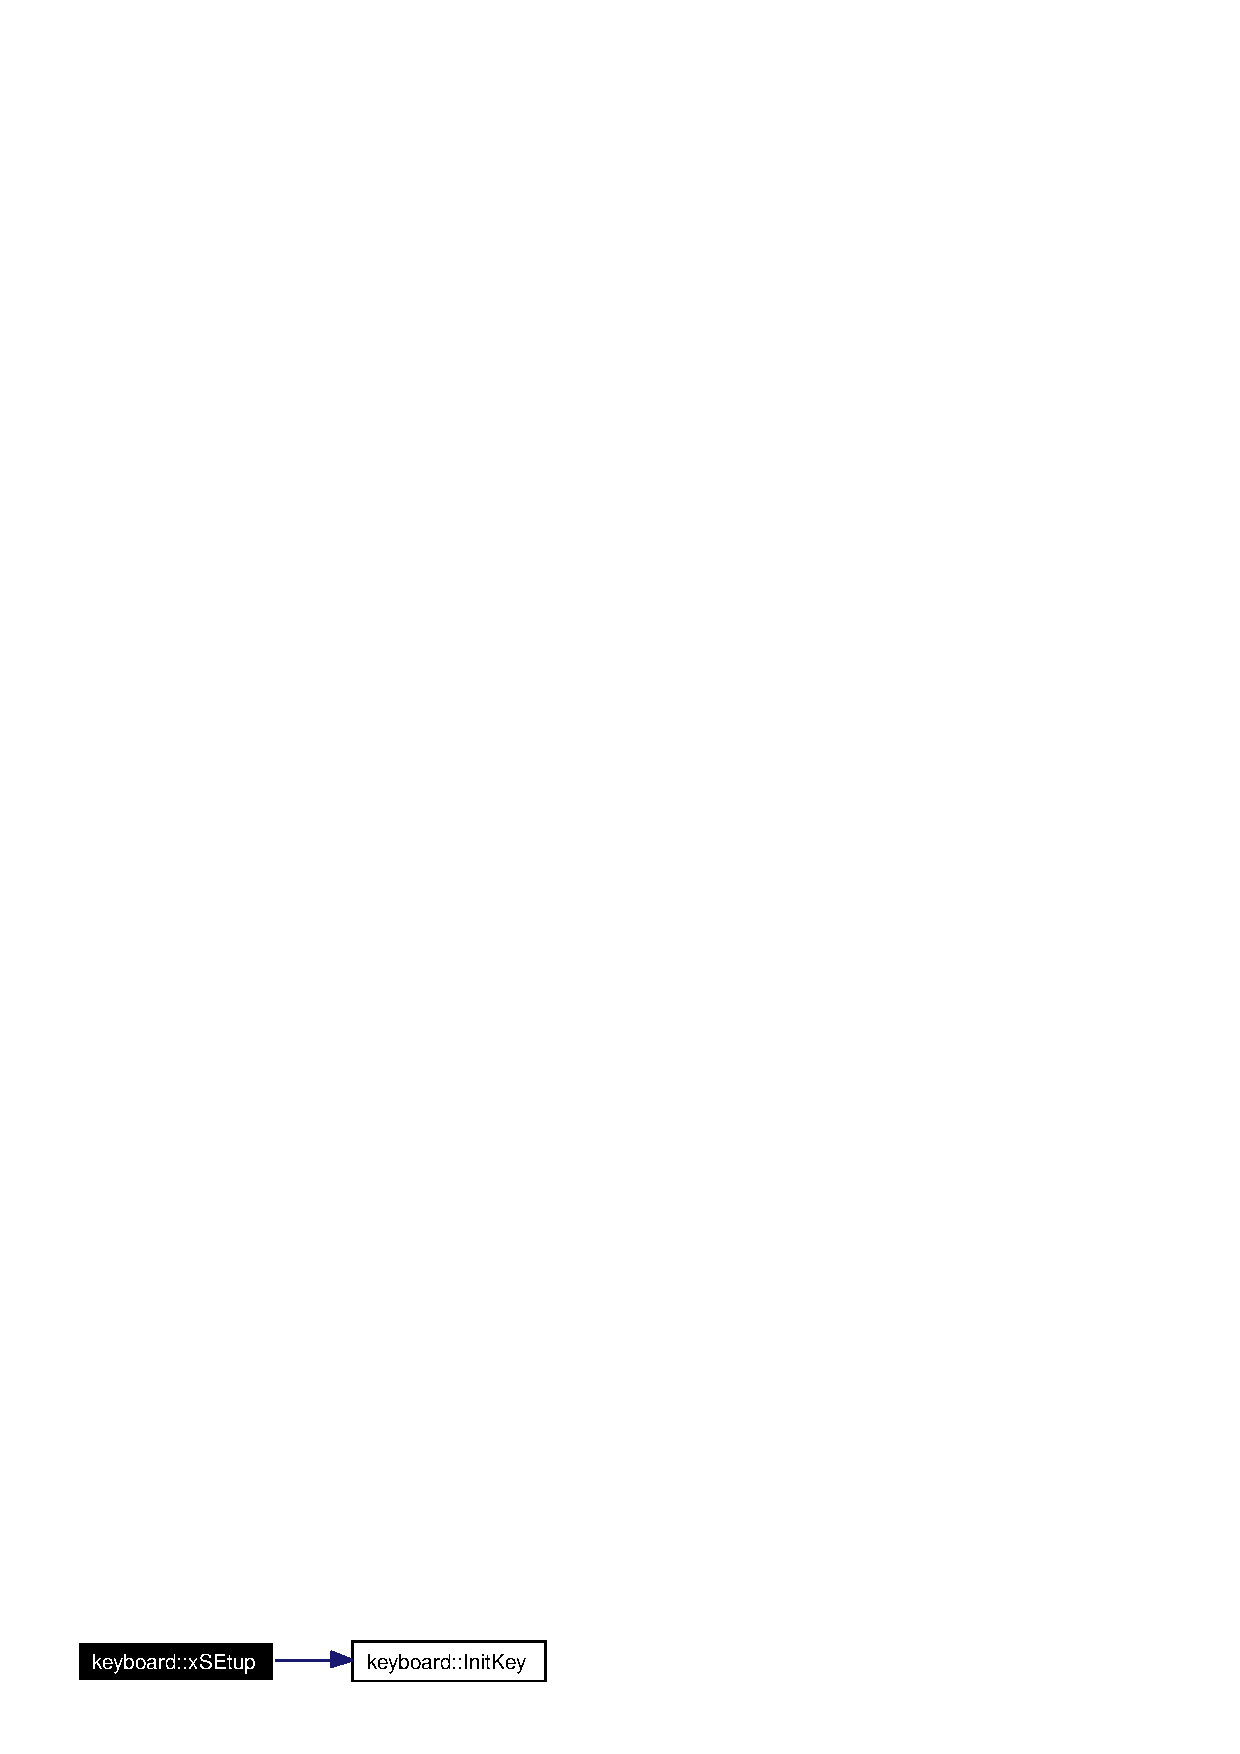
\includegraphics[width=131pt]{classkeyboard_keyboarda2_cgraph}
\end{center}
\end{figure}


\subsection{Member Data Documentation}
\index{keyboard@{keyboard}!key_0@{key\_\-0}}
\index{key_0@{key\_\-0}!keyboard@{keyboard}}
\subsubsection{\setlength{\rightskip}{0pt plus 5cm}{\bf keyboard\_\-key} $\ast$ {\bf keyboard::key\_\-0}\hspace{0.3cm}{\tt  [private]}}\label{classkeyboard_keyboardr35}




Definition at line 56 of file keyboard.h.

Referenced by Init\-Key().\index{keyboard@{keyboard}!key_1@{key\_\-1}}
\index{key_1@{key\_\-1}!keyboard@{keyboard}}
\subsubsection{\setlength{\rightskip}{0pt plus 5cm}{\bf keyboard\_\-key} $\ast$ {\bf keyboard::key\_\-1}\hspace{0.3cm}{\tt  [private]}}\label{classkeyboard_keyboardr26}




Definition at line 56 of file keyboard.h.

Referenced by Init\-Key().\index{keyboard@{keyboard}!key_2@{key\_\-2}}
\index{key_2@{key\_\-2}!keyboard@{keyboard}}
\subsubsection{\setlength{\rightskip}{0pt plus 5cm}{\bf keyboard\_\-key} $\ast$ {\bf keyboard::key\_\-2}\hspace{0.3cm}{\tt  [private]}}\label{classkeyboard_keyboardr27}




Definition at line 56 of file keyboard.h.

Referenced by Init\-Key().\index{keyboard@{keyboard}!key_3@{key\_\-3}}
\index{key_3@{key\_\-3}!keyboard@{keyboard}}
\subsubsection{\setlength{\rightskip}{0pt plus 5cm}{\bf keyboard\_\-key} $\ast$ {\bf keyboard::key\_\-3}\hspace{0.3cm}{\tt  [private]}}\label{classkeyboard_keyboardr28}




Definition at line 56 of file keyboard.h.

Referenced by Init\-Key().\index{keyboard@{keyboard}!key_4@{key\_\-4}}
\index{key_4@{key\_\-4}!keyboard@{keyboard}}
\subsubsection{\setlength{\rightskip}{0pt plus 5cm}{\bf keyboard\_\-key} $\ast$ {\bf keyboard::key\_\-4}\hspace{0.3cm}{\tt  [private]}}\label{classkeyboard_keyboardr29}




Definition at line 56 of file keyboard.h.

Referenced by Init\-Key().\index{keyboard@{keyboard}!key_5@{key\_\-5}}
\index{key_5@{key\_\-5}!keyboard@{keyboard}}
\subsubsection{\setlength{\rightskip}{0pt plus 5cm}{\bf keyboard\_\-key} $\ast$ {\bf keyboard::key\_\-5}\hspace{0.3cm}{\tt  [private]}}\label{classkeyboard_keyboardr30}




Definition at line 56 of file keyboard.h.

Referenced by Init\-Key().\index{keyboard@{keyboard}!key_6@{key\_\-6}}
\index{key_6@{key\_\-6}!keyboard@{keyboard}}
\subsubsection{\setlength{\rightskip}{0pt plus 5cm}{\bf keyboard\_\-key} $\ast$ {\bf keyboard::key\_\-6}\hspace{0.3cm}{\tt  [private]}}\label{classkeyboard_keyboardr31}




Definition at line 56 of file keyboard.h.

Referenced by Init\-Key().\index{keyboard@{keyboard}!key_7@{key\_\-7}}
\index{key_7@{key\_\-7}!keyboard@{keyboard}}
\subsubsection{\setlength{\rightskip}{0pt plus 5cm}{\bf keyboard\_\-key} $\ast$ {\bf keyboard::key\_\-7}\hspace{0.3cm}{\tt  [private]}}\label{classkeyboard_keyboardr32}




Definition at line 56 of file keyboard.h.

Referenced by Init\-Key().\index{keyboard@{keyboard}!key_8@{key\_\-8}}
\index{key_8@{key\_\-8}!keyboard@{keyboard}}
\subsubsection{\setlength{\rightskip}{0pt plus 5cm}{\bf keyboard\_\-key} $\ast$ {\bf keyboard::key\_\-8}\hspace{0.3cm}{\tt  [private]}}\label{classkeyboard_keyboardr33}




Definition at line 56 of file keyboard.h.

Referenced by Init\-Key().\index{keyboard@{keyboard}!key_9@{key\_\-9}}
\index{key_9@{key\_\-9}!keyboard@{keyboard}}
\subsubsection{\setlength{\rightskip}{0pt plus 5cm}{\bf keyboard\_\-key} $\ast$ {\bf keyboard::key\_\-9}\hspace{0.3cm}{\tt  [private]}}\label{classkeyboard_keyboardr34}




Definition at line 56 of file keyboard.h.

Referenced by Init\-Key().\index{keyboard@{keyboard}!key_a@{key\_\-a}}
\index{key_a@{key\_\-a}!keyboard@{keyboard}}
\subsubsection{\setlength{\rightskip}{0pt plus 5cm}{\bf keyboard\_\-key}$\ast$ {\bf keyboard::key\_\-a}\hspace{0.3cm}{\tt  [private]}}\label{classkeyboard_keyboardr0}




Definition at line 56 of file keyboard.h.

Referenced by Init\-Key().\index{keyboard@{keyboard}!key_b@{key\_\-b}}
\index{key_b@{key\_\-b}!keyboard@{keyboard}}
\subsubsection{\setlength{\rightskip}{0pt plus 5cm}{\bf keyboard\_\-key} $\ast$ {\bf keyboard::key\_\-b}\hspace{0.3cm}{\tt  [private]}}\label{classkeyboard_keyboardr1}




Definition at line 56 of file keyboard.h.

Referenced by Init\-Key().\index{keyboard@{keyboard}!key_backspace@{key\_\-backspace}}
\index{key_backspace@{key\_\-backspace}!keyboard@{keyboard}}
\subsubsection{\setlength{\rightskip}{0pt plus 5cm}{\bf keyboard\_\-key} $\ast$ {\bf keyboard::key\_\-backspace}\hspace{0.3cm}{\tt  [private]}}\label{classkeyboard_keyboardr40}




Definition at line 56 of file keyboard.h.

Referenced by Init\-Key().\index{keyboard@{keyboard}!key_c@{key\_\-c}}
\index{key_c@{key\_\-c}!keyboard@{keyboard}}
\subsubsection{\setlength{\rightskip}{0pt plus 5cm}{\bf keyboard\_\-key} $\ast$ {\bf keyboard::key\_\-c}\hspace{0.3cm}{\tt  [private]}}\label{classkeyboard_keyboardr2}




Definition at line 56 of file keyboard.h.

Referenced by Init\-Key().\index{keyboard@{keyboard}!key_change@{key\_\-change}}
\index{key_change@{key\_\-change}!keyboard@{keyboard}}
\subsubsection{\setlength{\rightskip}{0pt plus 5cm}{\bf keyboard\_\-key} $\ast$ {\bf keyboard::key\_\-change}\hspace{0.3cm}{\tt  [private]}}\label{classkeyboard_keyboardr39}




Definition at line 56 of file keyboard.h.

Referenced by Init\-Key().\index{keyboard@{keyboard}!key_comma@{key\_\-comma}}
\index{key_comma@{key\_\-comma}!keyboard@{keyboard}}
\subsubsection{\setlength{\rightskip}{0pt plus 5cm}{\bf keyboard\_\-key} $\ast$ {\bf keyboard::key\_\-comma}\hspace{0.3cm}{\tt  [private]}}\label{classkeyboard_keyboardr36}




Definition at line 56 of file keyboard.h.

Referenced by Init\-Key().\index{keyboard@{keyboard}!key_d@{key\_\-d}}
\index{key_d@{key\_\-d}!keyboard@{keyboard}}
\subsubsection{\setlength{\rightskip}{0pt plus 5cm}{\bf keyboard\_\-key} $\ast$ {\bf keyboard::key\_\-d}\hspace{0.3cm}{\tt  [private]}}\label{classkeyboard_keyboardr3}




Definition at line 56 of file keyboard.h.

Referenced by Init\-Key().\index{keyboard@{keyboard}!key_e@{key\_\-e}}
\index{key_e@{key\_\-e}!keyboard@{keyboard}}
\subsubsection{\setlength{\rightskip}{0pt plus 5cm}{\bf keyboard\_\-key} $\ast$ {\bf keyboard::key\_\-e}\hspace{0.3cm}{\tt  [private]}}\label{classkeyboard_keyboardr4}




Definition at line 56 of file keyboard.h.

Referenced by Init\-Key().\index{keyboard@{keyboard}!key_enter@{key\_\-enter}}
\index{key_enter@{key\_\-enter}!keyboard@{keyboard}}
\subsubsection{\setlength{\rightskip}{0pt plus 5cm}{\bf keyboard\_\-key} $\ast$ {\bf keyboard::key\_\-enter}\hspace{0.3cm}{\tt  [private]}}\label{classkeyboard_keyboardr38}




Definition at line 56 of file keyboard.h.

Referenced by Init\-Key().\index{keyboard@{keyboard}!key_f@{key\_\-f}}
\index{key_f@{key\_\-f}!keyboard@{keyboard}}
\subsubsection{\setlength{\rightskip}{0pt plus 5cm}{\bf keyboard\_\-key} $\ast$ {\bf keyboard::key\_\-f}\hspace{0.3cm}{\tt  [private]}}\label{classkeyboard_keyboardr5}




Definition at line 56 of file keyboard.h.

Referenced by Init\-Key().\index{keyboard@{keyboard}!key_g@{key\_\-g}}
\index{key_g@{key\_\-g}!keyboard@{keyboard}}
\subsubsection{\setlength{\rightskip}{0pt plus 5cm}{\bf keyboard\_\-key} $\ast$ {\bf keyboard::key\_\-g}\hspace{0.3cm}{\tt  [private]}}\label{classkeyboard_keyboardr6}




Definition at line 56 of file keyboard.h.

Referenced by Init\-Key().\index{keyboard@{keyboard}!key_h@{key\_\-h}}
\index{key_h@{key\_\-h}!keyboard@{keyboard}}
\subsubsection{\setlength{\rightskip}{0pt plus 5cm}{\bf keyboard\_\-key} $\ast$ {\bf keyboard::key\_\-h}\hspace{0.3cm}{\tt  [private]}}\label{classkeyboard_keyboardr7}




Definition at line 56 of file keyboard.h.

Referenced by Init\-Key().\index{keyboard@{keyboard}!key_i@{key\_\-i}}
\index{key_i@{key\_\-i}!keyboard@{keyboard}}
\subsubsection{\setlength{\rightskip}{0pt plus 5cm}{\bf keyboard\_\-key} $\ast$ {\bf keyboard::key\_\-i}\hspace{0.3cm}{\tt  [private]}}\label{classkeyboard_keyboardr8}




Definition at line 56 of file keyboard.h.

Referenced by Init\-Key().\index{keyboard@{keyboard}!key_j@{key\_\-j}}
\index{key_j@{key\_\-j}!keyboard@{keyboard}}
\subsubsection{\setlength{\rightskip}{0pt plus 5cm}{\bf keyboard\_\-key} $\ast$ {\bf keyboard::key\_\-j}\hspace{0.3cm}{\tt  [private]}}\label{classkeyboard_keyboardr9}




Definition at line 56 of file keyboard.h.

Referenced by Init\-Key().\index{keyboard@{keyboard}!key_k@{key\_\-k}}
\index{key_k@{key\_\-k}!keyboard@{keyboard}}
\subsubsection{\setlength{\rightskip}{0pt plus 5cm}{\bf keyboard\_\-key} $\ast$ {\bf keyboard::key\_\-k}\hspace{0.3cm}{\tt  [private]}}\label{classkeyboard_keyboardr10}




Definition at line 56 of file keyboard.h.

Referenced by Init\-Key().\index{keyboard@{keyboard}!key_l@{key\_\-l}}
\index{key_l@{key\_\-l}!keyboard@{keyboard}}
\subsubsection{\setlength{\rightskip}{0pt plus 5cm}{\bf keyboard\_\-key} $\ast$ {\bf keyboard::key\_\-l}\hspace{0.3cm}{\tt  [private]}}\label{classkeyboard_keyboardr11}




Definition at line 56 of file keyboard.h.

Referenced by Init\-Key().\index{keyboard@{keyboard}!key_list@{key\_\-list}}
\index{key_list@{key\_\-list}!keyboard@{keyboard}}
\subsubsection{\setlength{\rightskip}{0pt plus 5cm}QPtr\-List$<${\bf keyboard\_\-key}$>$ {\bf keyboard::key\_\-list}\hspace{0.3cm}{\tt  [private]}}\label{classkeyboard_keyboardr45}




Definition at line 62 of file keyboard.h.

Referenced by Init\-Key(), and slot\-Change().\index{keyboard@{keyboard}!key_m@{key\_\-m}}
\index{key_m@{key\_\-m}!keyboard@{keyboard}}
\subsubsection{\setlength{\rightskip}{0pt plus 5cm}{\bf keyboard\_\-key} $\ast$ {\bf keyboard::key\_\-m}\hspace{0.3cm}{\tt  [private]}}\label{classkeyboard_keyboardr12}




Definition at line 56 of file keyboard.h.

Referenced by Init\-Key().\index{keyboard@{keyboard}!key_n@{key\_\-n}}
\index{key_n@{key\_\-n}!keyboard@{keyboard}}
\subsubsection{\setlength{\rightskip}{0pt plus 5cm}{\bf keyboard\_\-key} $\ast$ {\bf keyboard::key\_\-n}\hspace{0.3cm}{\tt  [private]}}\label{classkeyboard_keyboardr13}




Definition at line 56 of file keyboard.h.

Referenced by Init\-Key().\index{keyboard@{keyboard}!key_o@{key\_\-o}}
\index{key_o@{key\_\-o}!keyboard@{keyboard}}
\subsubsection{\setlength{\rightskip}{0pt plus 5cm}{\bf keyboard\_\-key} $\ast$ {\bf keyboard::key\_\-o}\hspace{0.3cm}{\tt  [private]}}\label{classkeyboard_keyboardr14}




Definition at line 56 of file keyboard.h.

Referenced by Init\-Key().\index{keyboard@{keyboard}!key_p@{key\_\-p}}
\index{key_p@{key\_\-p}!keyboard@{keyboard}}
\subsubsection{\setlength{\rightskip}{0pt plus 5cm}{\bf keyboard\_\-key} $\ast$ {\bf keyboard::key\_\-p}\hspace{0.3cm}{\tt  [private]}}\label{classkeyboard_keyboardr15}




Definition at line 56 of file keyboard.h.

Referenced by Init\-Key().\index{keyboard@{keyboard}!key_q@{key\_\-q}}
\index{key_q@{key\_\-q}!keyboard@{keyboard}}
\subsubsection{\setlength{\rightskip}{0pt plus 5cm}{\bf keyboard\_\-key} $\ast$ {\bf keyboard::key\_\-q}\hspace{0.3cm}{\tt  [private]}}\label{classkeyboard_keyboardr16}




Definition at line 56 of file keyboard.h.

Referenced by Init\-Key().\index{keyboard@{keyboard}!key_r@{key\_\-r}}
\index{key_r@{key\_\-r}!keyboard@{keyboard}}
\subsubsection{\setlength{\rightskip}{0pt plus 5cm}{\bf keyboard\_\-key} $\ast$ {\bf keyboard::key\_\-r}\hspace{0.3cm}{\tt  [private]}}\label{classkeyboard_keyboardr17}




Definition at line 56 of file keyboard.h.

Referenced by Init\-Key().\index{keyboard@{keyboard}!key_s@{key\_\-s}}
\index{key_s@{key\_\-s}!keyboard@{keyboard}}
\subsubsection{\setlength{\rightskip}{0pt plus 5cm}{\bf keyboard\_\-key} $\ast$ {\bf keyboard::key\_\-s}\hspace{0.3cm}{\tt  [private]}}\label{classkeyboard_keyboardr18}




Definition at line 56 of file keyboard.h.

Referenced by Init\-Key().\index{keyboard@{keyboard}!key_space@{key\_\-space}}
\index{key_space@{key\_\-space}!keyboard@{keyboard}}
\subsubsection{\setlength{\rightskip}{0pt plus 5cm}{\bf keyboard\_\-key} $\ast$ {\bf keyboard::key\_\-space}\hspace{0.3cm}{\tt  [private]}}\label{classkeyboard_keyboardr37}




Definition at line 56 of file keyboard.h.

Referenced by Init\-Key().\index{keyboard@{keyboard}!key_t@{key\_\-t}}
\index{key_t@{key\_\-t}!keyboard@{keyboard}}
\subsubsection{\setlength{\rightskip}{0pt plus 5cm}{\bf keyboard\_\-key} $\ast$ {\bf keyboard::key\_\-t}\hspace{0.3cm}{\tt  [private]}}\label{classkeyboard_keyboardr19}




Definition at line 56 of file keyboard.h.

Referenced by Init\-Key().\index{keyboard@{keyboard}!key_u@{key\_\-u}}
\index{key_u@{key\_\-u}!keyboard@{keyboard}}
\subsubsection{\setlength{\rightskip}{0pt plus 5cm}{\bf keyboard\_\-key} $\ast$ {\bf keyboard::key\_\-u}\hspace{0.3cm}{\tt  [private]}}\label{classkeyboard_keyboardr20}




Definition at line 56 of file keyboard.h.

Referenced by Init\-Key().\index{keyboard@{keyboard}!key_v@{key\_\-v}}
\index{key_v@{key\_\-v}!keyboard@{keyboard}}
\subsubsection{\setlength{\rightskip}{0pt plus 5cm}{\bf keyboard\_\-key} $\ast$ {\bf keyboard::key\_\-v}\hspace{0.3cm}{\tt  [private]}}\label{classkeyboard_keyboardr21}




Definition at line 56 of file keyboard.h.

Referenced by Init\-Key().\index{keyboard@{keyboard}!key_w@{key\_\-w}}
\index{key_w@{key\_\-w}!keyboard@{keyboard}}
\subsubsection{\setlength{\rightskip}{0pt plus 5cm}{\bf keyboard\_\-key} $\ast$ {\bf keyboard::key\_\-w}\hspace{0.3cm}{\tt  [private]}}\label{classkeyboard_keyboardr22}




Definition at line 56 of file keyboard.h.

Referenced by Init\-Key().\index{keyboard@{keyboard}!key_x@{key\_\-x}}
\index{key_x@{key\_\-x}!keyboard@{keyboard}}
\subsubsection{\setlength{\rightskip}{0pt plus 5cm}{\bf keyboard\_\-key} $\ast$ {\bf keyboard::key\_\-x}\hspace{0.3cm}{\tt  [private]}}\label{classkeyboard_keyboardr23}




Definition at line 56 of file keyboard.h.

Referenced by Init\-Key().\index{keyboard@{keyboard}!key_y@{key\_\-y}}
\index{key_y@{key\_\-y}!keyboard@{keyboard}}
\subsubsection{\setlength{\rightskip}{0pt plus 5cm}{\bf keyboard\_\-key} $\ast$ {\bf keyboard::key\_\-y}\hspace{0.3cm}{\tt  [private]}}\label{classkeyboard_keyboardr24}




Definition at line 56 of file keyboard.h.

Referenced by Init\-Key().\index{keyboard@{keyboard}!key_z@{key\_\-z}}
\index{key_z@{key\_\-z}!keyboard@{keyboard}}
\subsubsection{\setlength{\rightskip}{0pt plus 5cm}{\bf keyboard\_\-key} $\ast$ {\bf keyboard::key\_\-z}\hspace{0.3cm}{\tt  [private]}}\label{classkeyboard_keyboardr25}




Definition at line 56 of file keyboard.h.

Referenced by Init\-Key().\index{keyboard@{keyboard}!Label@{Label}}
\index{Label@{Label}!keyboard@{keyboard}}
\subsubsection{\setlength{\rightskip}{0pt plus 5cm}QLabel$\ast$ {\bf keyboard::Label}\hspace{0.3cm}{\tt  [private]}}\label{classkeyboard_keyboardr43}




Definition at line 60 of file keyboard.h.

Referenced by Init\-Key(), and slot\-Receive\-Char().\index{keyboard@{keyboard}!pixBackground@{pixBackground}}
\index{pixBackground@{pixBackground}!keyboard@{keyboard}}
\subsubsection{\setlength{\rightskip}{0pt plus 5cm}QPixmap {\bf keyboard::pix\-Background}\hspace{0.3cm}{\tt  [private]}}\label{classkeyboard_keyboardr41}




Definition at line 57 of file keyboard.h.\index{keyboard@{keyboard}!pixMask@{pixMask}}
\index{pixMask@{pixMask}!keyboard@{keyboard}}
\subsubsection{\setlength{\rightskip}{0pt plus 5cm}QBitmap {\bf keyboard::pix\-Mask}\hspace{0.3cm}{\tt  [private]}}\label{classkeyboard_keyboardr42}




Definition at line 58 of file keyboard.h.

Referenced by x\-SEtup().\index{keyboard@{keyboard}!strString@{strString}}
\index{strString@{strString}!keyboard@{keyboard}}
\subsubsection{\setlength{\rightskip}{0pt plus 5cm}QString {\bf keyboard::str\-String}}\label{classkeyboard_keyboardo0}




Definition at line 44 of file keyboard.h.

Referenced by slot\-Clear\-Str(), slot\-Receive\-Char(), and slot\-Send\-String().\index{keyboard@{keyboard}!upper@{upper}}
\index{upper@{upper}!keyboard@{keyboard}}
\subsubsection{\setlength{\rightskip}{0pt plus 5cm}bool {\bf keyboard::upper}\hspace{0.3cm}{\tt  [private]}}\label{classkeyboard_keyboardr44}




Definition at line 61 of file keyboard.h.

Referenced by slot\-Change(), and x\-SEtup().

The documentation for this class was generated from the following files:\begin{CompactItemize}
\item 
{\bf keyboard.h}\item 
{\bf keyboard.moc}\item 
{\bf keyboard.cpp}\end{CompactItemize}
